\section*{Formatting examples}

This section provides examples of \LaTeX{} tables, figures, equations,
lists, citations, and references to the same. This will not be compiled if
the WIP flag is not set.
\subsection*{Text}

Use \verb|\textbf{}| to \textbf{bold text}, \verb|\textit{}| to
\textit{italicize}, \verb|\verb||| for \verb|code|, or one after the other for
\textit{\textbf{both}}.
If there is no blank line or explicit newline after the previous thing, you're
in the same paragraph. Without a blank line or newline, the paragraph will be
continuous.

Blank line for a new paragraph (you know because it's automatically indented).
Two backslashes \verb|\\| \\ for a new line without a new paragraph.

Backslash open/close parentheses for inline equations \(\omega = \Omega \equiv
\sqrt{\frac{k}{m}}\). Greek letters are just their English spelling, and capital
Greek letters capitalize the first letter. Aligned non-numbered equation using
brackets:

\[f(t) = \sum_{k = 0}^{\infty} a_{n} \sin(k\omega_{0}x)\]

\subsection*{Lists}

\begin{enumerate}[(1)]
    \item \verb|\begin{enumerate}[<format>] .. \item ... \end{enumerate}| to create a list. \label{list:examples-head}

    \item This list has the format \verb|(1)|, which means it will be numbered, with parentheses surrounding the number.

    \item 
\end{enumerate}

\subsection*{Figures and tables}
Aligned numbered equation (Eq. \ref{eq:example-eq}) using \verb|begin| and \verb|end|:

\subsection*{Cross-references}

\verb|\[ ... \]| creates an aligned unlabeled equation. To make a labeled equation, create an \verb|equation| environment: 

\begin{equation} \label{eq:example-eq}
    f(t) = \sum_{k = 0}^{\infty} a_{n} \sin(k\omega_{0}x)
\end{equation}

To cite Eq. \ref{eq:example-eq}, use \verb|\ref{}|. Figures and tables each have
their own numbering, and you can refer to them with  Fig. \ref{fig:example-fig},
Table \ref{tbl:example-table}. You can also refer to list items, like item
\ref{list:examples-head}, which is the list item for creating lists.


\begin{figure}[H]
    \centering
    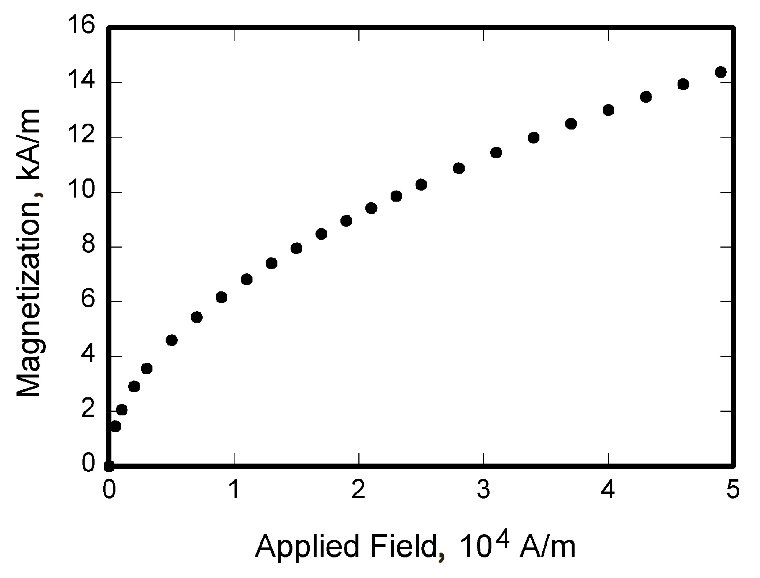
\includegraphics[width=2in]{fig/graph.jpg} % path to figure
    \caption{Magnetization as a function of applied fields} 
    \label{fig:example-fig} % how we refer to this figure's number
    % Figures must have "fig:" in the label and tables must have "tbl:" in
    % the label
\end{figure}

\begin{table}[H]
    \centering
    \caption{Informative table caption}
    % in this case, Tabular is how we express a table in LaTeX, but if we
    % had a picture of a table, we would include that using \includegraphics
    % or similar.

    % the vertical bars you put in the spec will appear - if you want two
    % columns to not be separated, omit that bar.
    \begin{tabular}{|l|cr|p{2in}|} 

        % MANDATORY: Each table row starts with "\hline" and ends with "\\"
        \hline Left column & Centered column & Right column & 2" fixed-width
        column \\
        \hline A & B & C & Lorem ipsum dolor sit amet, consectetur adipiscing elit \\
        \hline D & E & F & sed do eiusmod tempor incididunt ut labore et
        dolore magna aliqua \\
        \hline % MANDATORY: Table ends with one "\hline"
    \end{tabular}	
    \label{tbl:example-table}
\end{table}	

\paragraph{Citations} Use the \verb|cite| command to cite resources in the
\verb|.bib| file \cite{peyret2012computational, oates1997aerothermodynamics}.